
\section{Wyniki optymalizacji}

Poniżej zamieszczamy wyniki przeprowadzonych przez nas testów.
Dla każdego testu prezentujemy wykorzystane dane (parametry procesorów i łącz),
wyniki optymalizacji oraz wykres Gantta.
Przygotowaliśmy 3 testy dla modeli sekwencyjnych i 2 testy dla modeli równoległych. \\

W każdym z poniższych testów przyjmujemy zerowy czas rozpoczęcia transmisji na łączu w celu uproszczenia wyników. \\

Na poniższych wykresach Gantta ciemny kolor oznacza obliczenia, natomiast jaśniejsze kolory o podobnych odcieniach oznaczają komunikację między danymi procesorami.

\subsection{Pierwszy test systemu sekwencyjnego} \label{test1}

\begin{table}[H]
\begin{minipage}[b]{0.5\linewidth}
\centering
\begin{tabular}{c l}
$V$ & 200 \\
$A1$ & 20 \\
$A2$ & 10 \\
$A3$ & 25 \\
$A4$ & 10 \\
$S12$ & 0 \\
$S23$ & 0 \\
$S34$ & 0 \\
$S24$ & 0 \\
$C12$ & 2 \\
$C23$ & 3 \\
$C34$ & 3 \\
$C24$ & 7 \\
\end{tabular}
\end{minipage}
\hspace{0.5cm}
\begin{minipage}[b]{0.5\linewidth}
\centering
\begin{tabular}{c l}
$T$ & 1275 \\
$d_{1}$ & 48 \\
$d_{2}$ & 72 \\
$d_{3}$ & 22 \\
$d_{4}$ & 57 \\
$d_{43}$ & 56 \\
$d_{42}$ & 1 \\
$t_{k12}$ & 304 \\
$t_{k23}$ & 234 \\
$t_{k24}$ & 7 \\
$t_{k34}$ & 168 \\
\end{tabular}
\end{minipage}
\caption{Dane wejściowe i wyniki optymalizacji testu~\ref{test1}}
\label{tab:res_1a}
\end{table}

\begin{figure}[H]
\centering
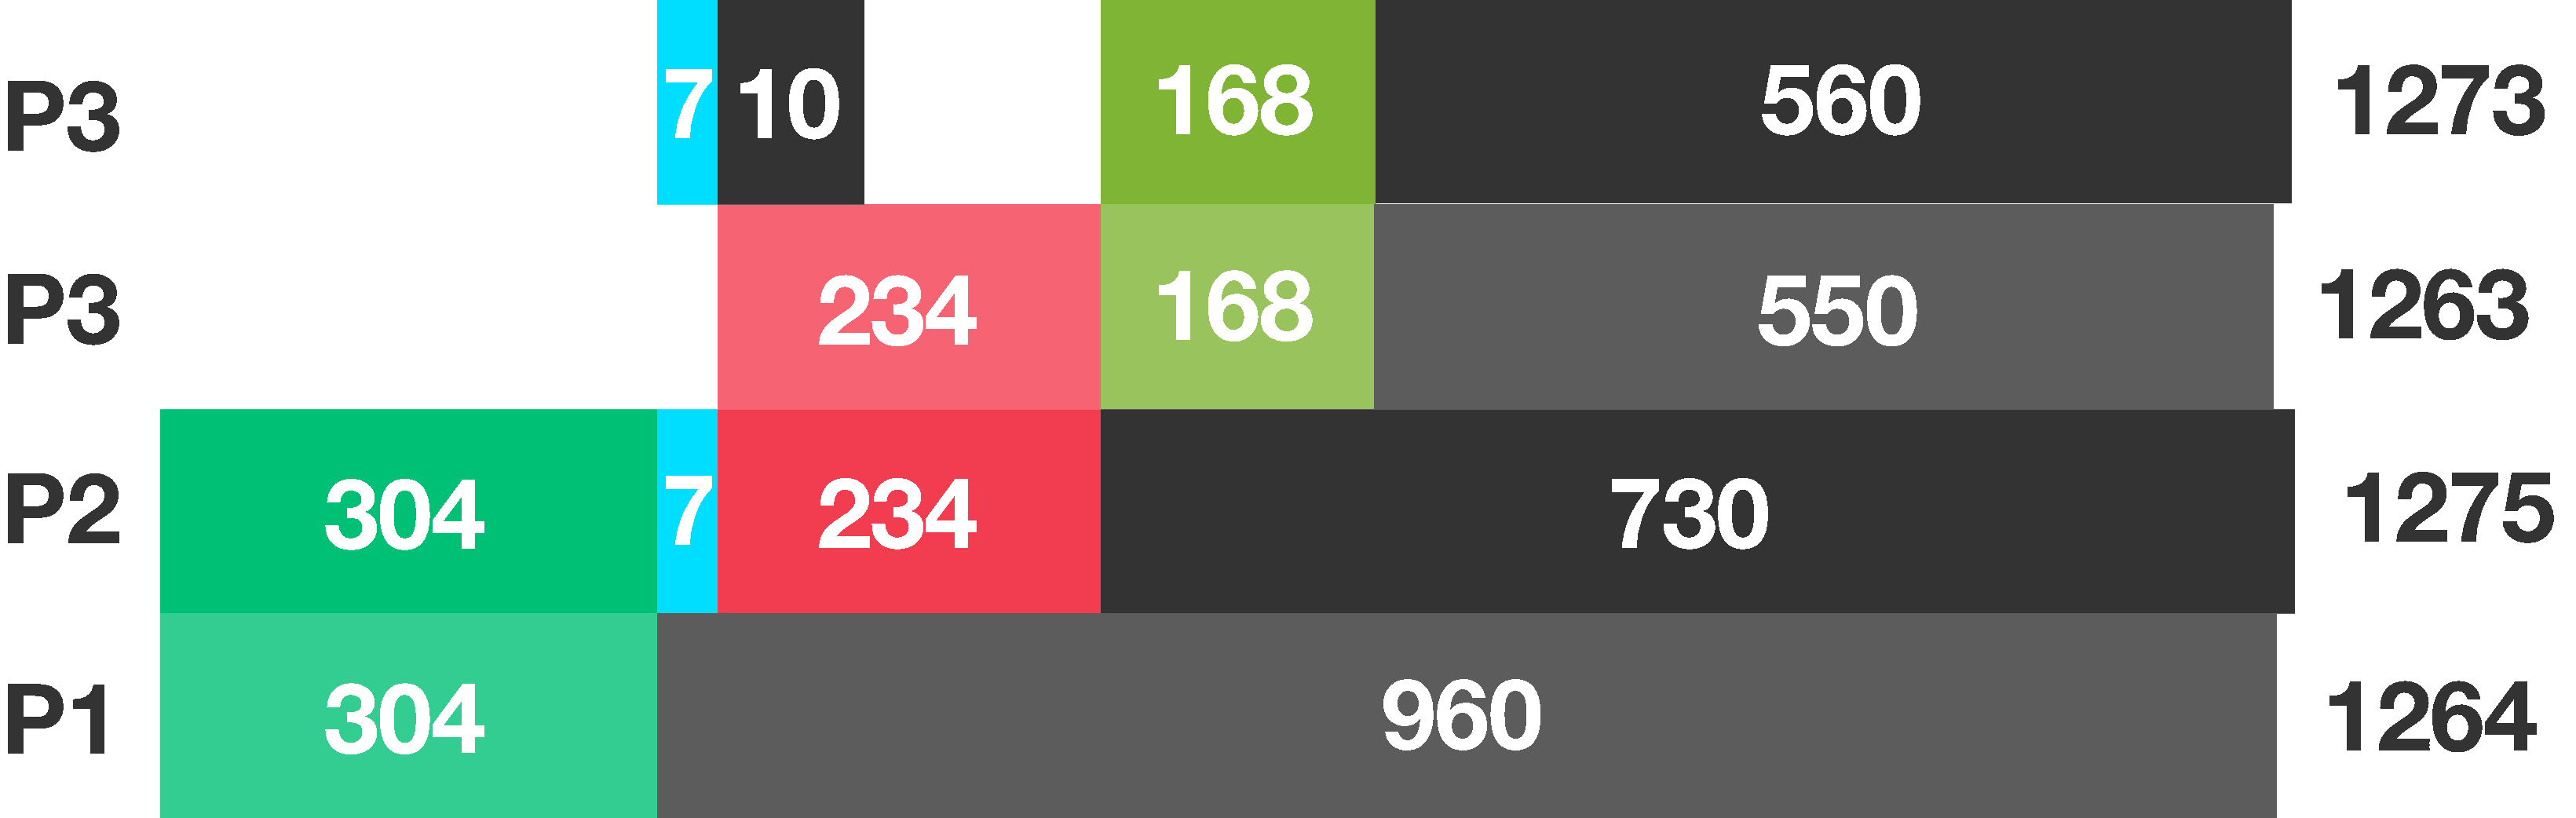
\includegraphics[width=1.0\textwidth]{g_sek1.pdf}
\caption{Wykres Gantta dla testu~\ref{test1}}
\label{fig:res_1b}
\end{figure}

\subsection{Drugi test systemu sekwencyjnego} \label{test2}

\begin{table}[H]
\begin{minipage}[b]{0.5\linewidth}
\centering
\begin{tabular}{c l}
$V$ & 200 \\
$A1$ & 20 \\
$A2$ & 30 \\
$A3$ & 25 \\
$A4$ & 5 \\
$S12$ & 0 \\
$S23$ & 0 \\
$S34$ & 0 \\
$S24$ & 0 \\
$C12$ & 2 \\
$C23$ & 5 \\
$C34$ & 3 \\
$C24$ & 10 \\
\end{tabular}
\end{minipage}
\hspace{0.5cm}
\begin{minipage}[b]{0.5\linewidth}
\centering
\begin{tabular}{c l}
$T$ & 1570 \\
$d_{1}$ & 65 \\
$d_{2}$ & 23 \\
$d_{3}$ & 22 \\
$d_{4}$ & 90 \\
$d_{43}$ & 80 \\
$d_{42}$ & 10 \\
$t_{k12}$ & 270 \\
$t_{k23}$ & 510 \\
$t_{k24}$ & 100 \\
$t_{k34}$ & 240 \\
\end{tabular}
\end{minipage}
\caption{Dane wejściowe i wyniki optymalizacji testu~\ref{test2}}
\label{tab:res_2a}
\end{table}

\begin{figure}[H]
\centering
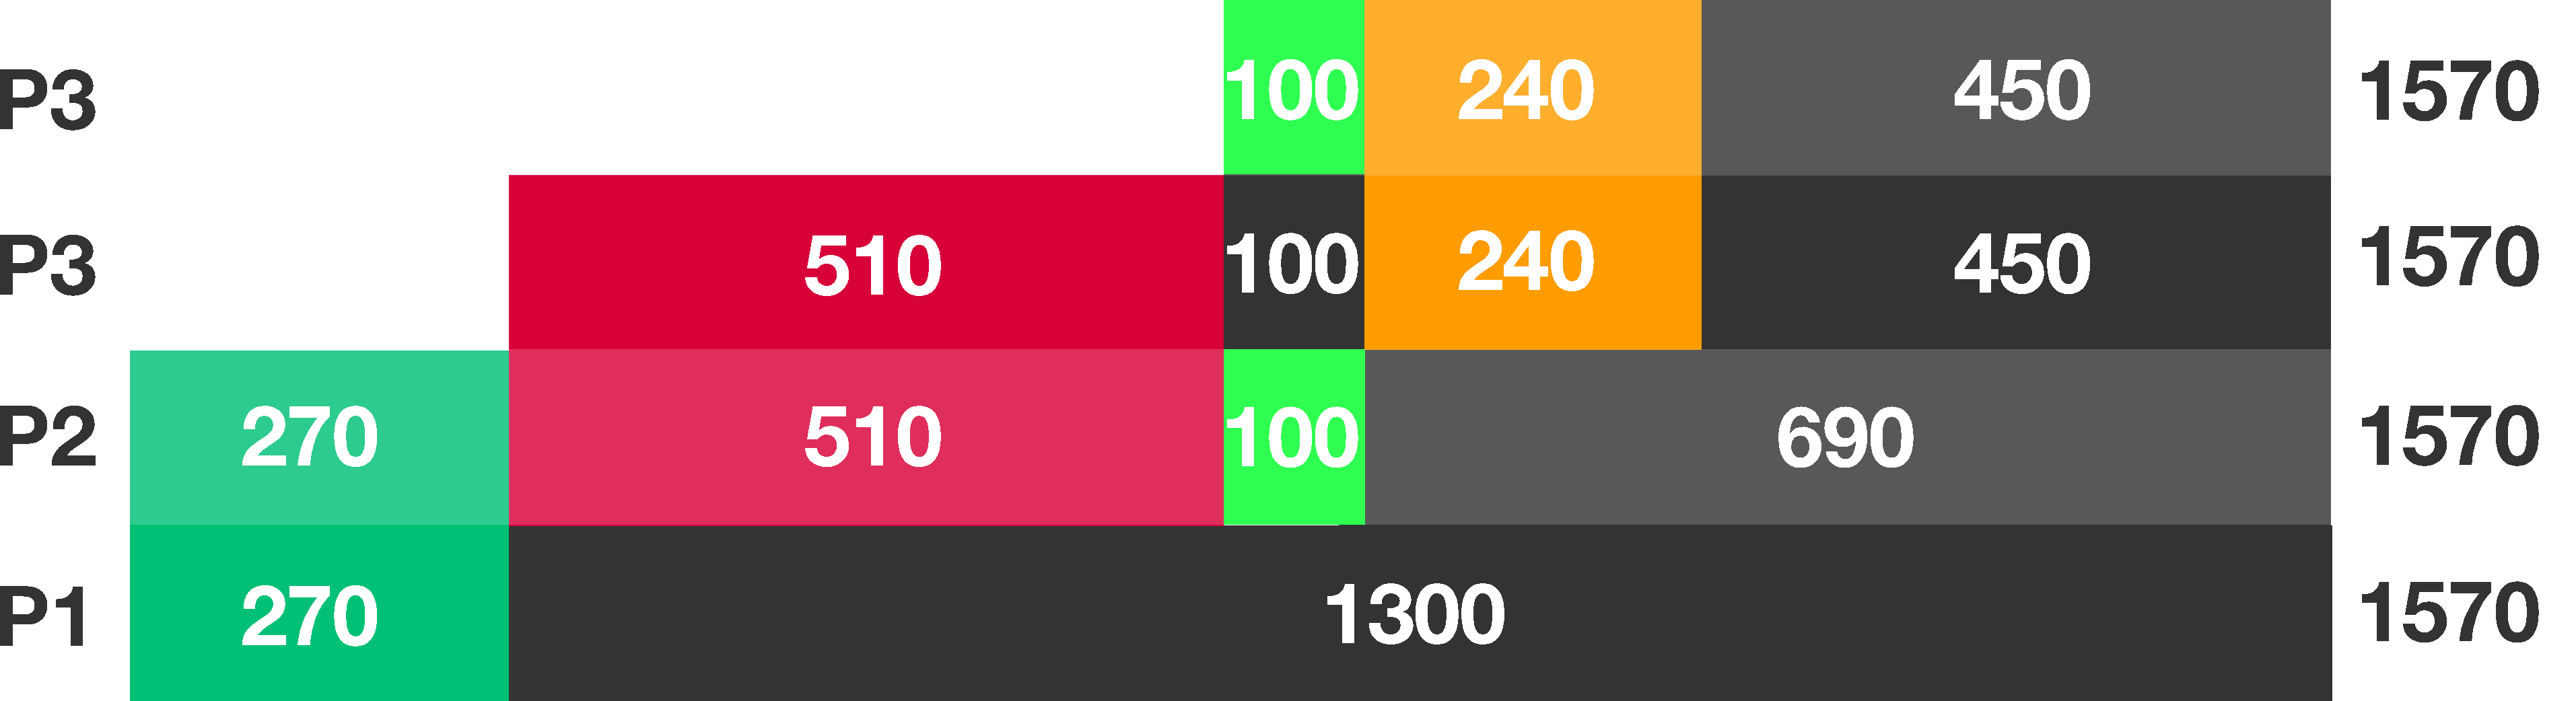
\includegraphics[width=1.0\textwidth]{g_sek3.pdf}
\caption{Wykres Gantta dla testu~\ref{test2}}
\label{fig:res_2b}
\end{figure}

\subsection{Trzeci test systemu sekwencyjnego} \label{test3}

\begin{table}[H]
\begin{minipage}[b]{0.5\linewidth}
\centering
\begin{tabular}{c l}
$V$ & 200 \\
$A1$ & 20 \\
$A2$ & 10 \\
$A3$ & 25 \\
$A4$ & 10 \\
$S12$ & 0 \\
$S23$ & 0 \\
$S34$ & 0 \\
$S24$ & 0 \\
$C12$ & 2 \\
$C23$ & 2 \\
$C34$ & 2 \\
$C24$ & 7 \\
\end{tabular}
\end{minipage}
\hspace{0.5cm}
\begin{minipage}[b]{0.5\linewidth}
\centering
\begin{tabular}{c l}
$T$ & 1277 \\
$d_{1}$ & 48 \\
$d_{2}$ & 83 \\
$d_{3}$ & 20 \\
$d_{4}$ & 49 \\
$d_{43}$ & 48 \\
$d_{42}$ & 1 \\
$t_{k12}$ & 304 \\
$t_{k23}$ & 136 \\
$t_{k24}$ & 7 \\
$t_{k34}$ & 336 \\
\end{tabular}
\end{minipage}
\caption{Dane wejściowe i wyniki optymalizacji testu~\ref{test3}}
\label{tab:res_3a}
\end{table}

\begin{figure}[H]
\centering
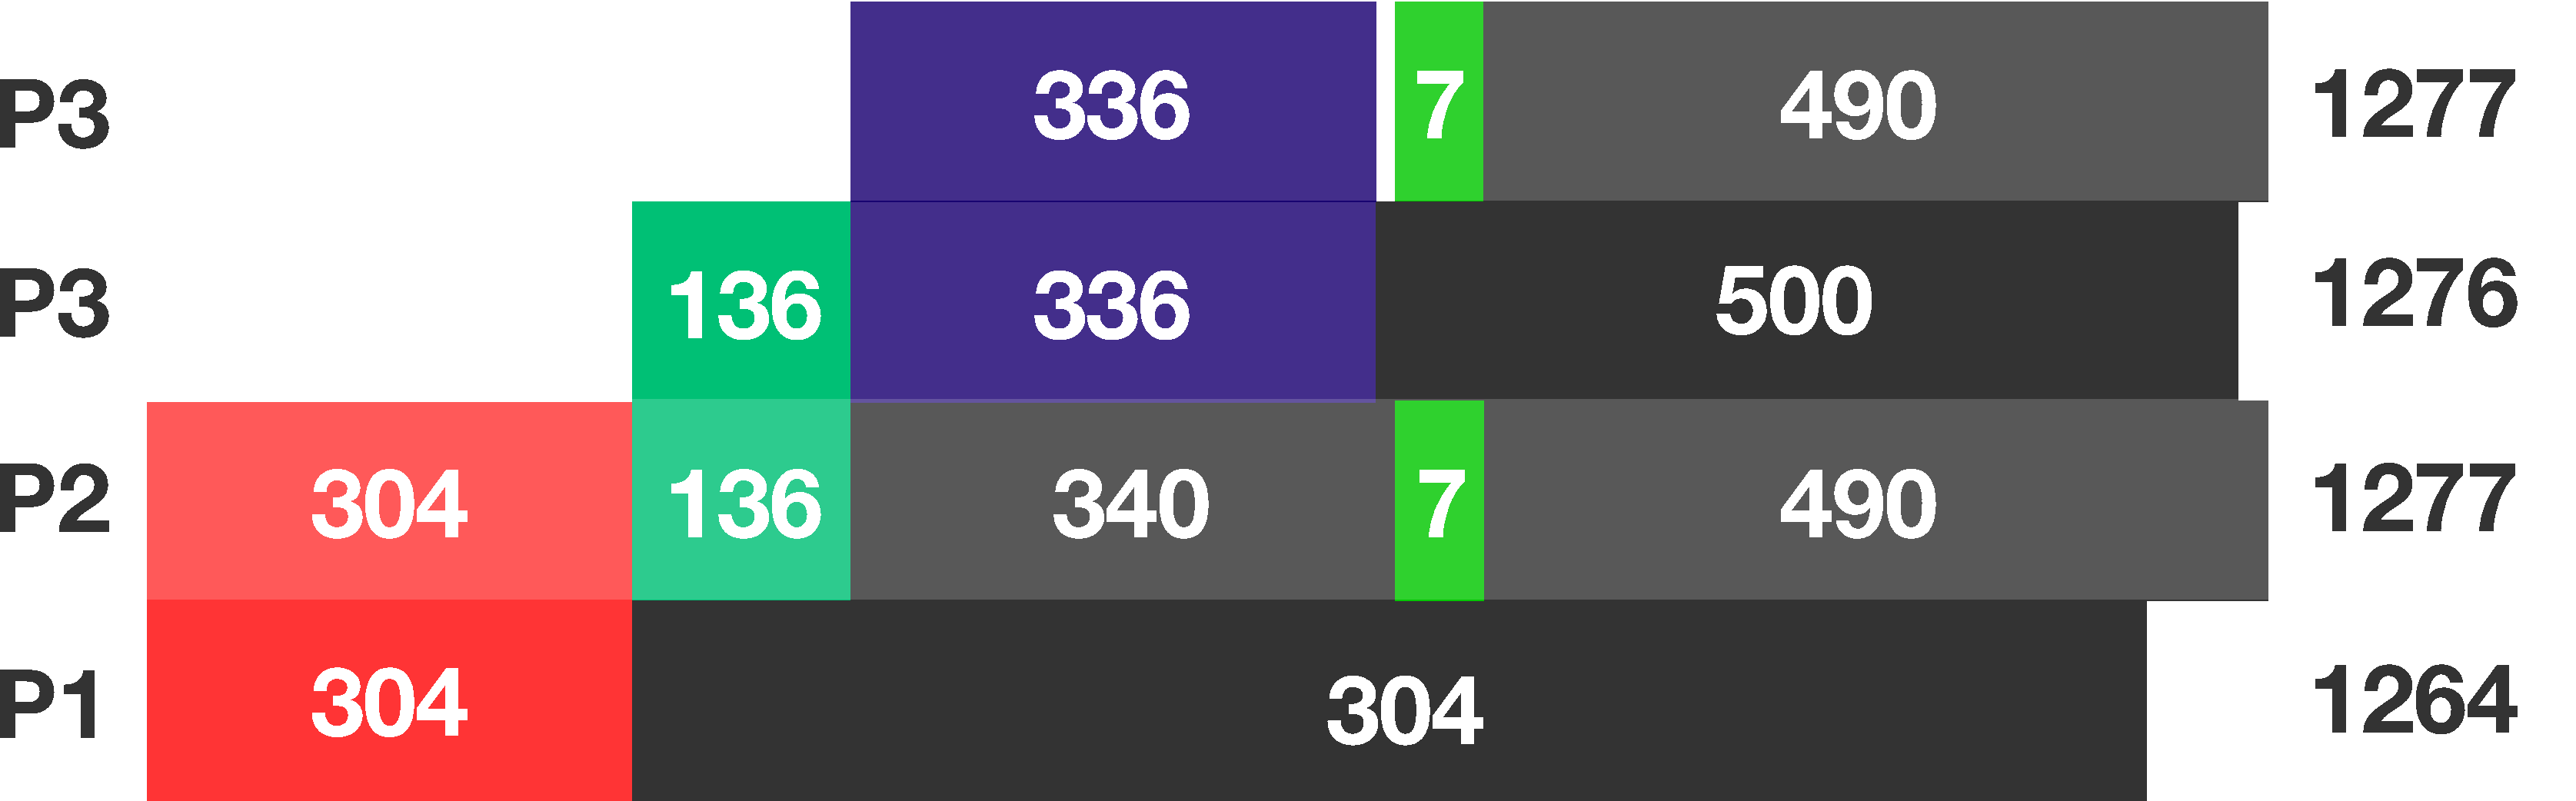
\includegraphics[width=1.0\textwidth]{g_sek2.pdf}
\caption{Wykres Gantta dla testu~\ref{test3}}
\label{fig:res_3b}
\end{figure}



\subsection{Pierwszy test systemu równoległego} \label{test4}

\begin{table}[H]
\begin{minipage}[b]{0.5\linewidth}
\centering
\begin{tabular}{c l}
$V$ & 200 \\
$A1$ & 100 \\
$A2$ & 10 \\
$A3$ & 100 \\
$A4$ & 10 \\
$S12$ & 0 \\
$S23$ & 0 \\
$S34$ & 0 \\
$S24$ & 0 \\
$C12$ & 2 \\
$C23$ & 4 \\
$C34$ & 2 \\
$C24$ & 4 \\
\end{tabular}
\end{minipage}
\hspace{0.5cm}
\begin{minipage}[b]{0.5\linewidth}
\centering
\begin{tabular}{c l}
$T$ & 1334 \\
$d_{1}$ & 13 \\
$d_{2}$ & 96 \\
$d_{3}$ & 7 \\
$d_{4}$ & 84 \\
$d_{43}$ & 54 \\
$d_{42}$ & 30 \\
$t_{k12}$ & 374 \\
$t_{k23}$ & 244 \\
$t_{k24}$ & 120 \\
$t_{k34}$ & 108 \\
$bg24$ & 0 \\
\end{tabular}
\end{minipage}
\caption{Dane wejściowe i wyniki optymalizacji testu~\ref{test4}}
\label{tab:res_4a}
\end{table}

\begin{figure}[H]
\centering
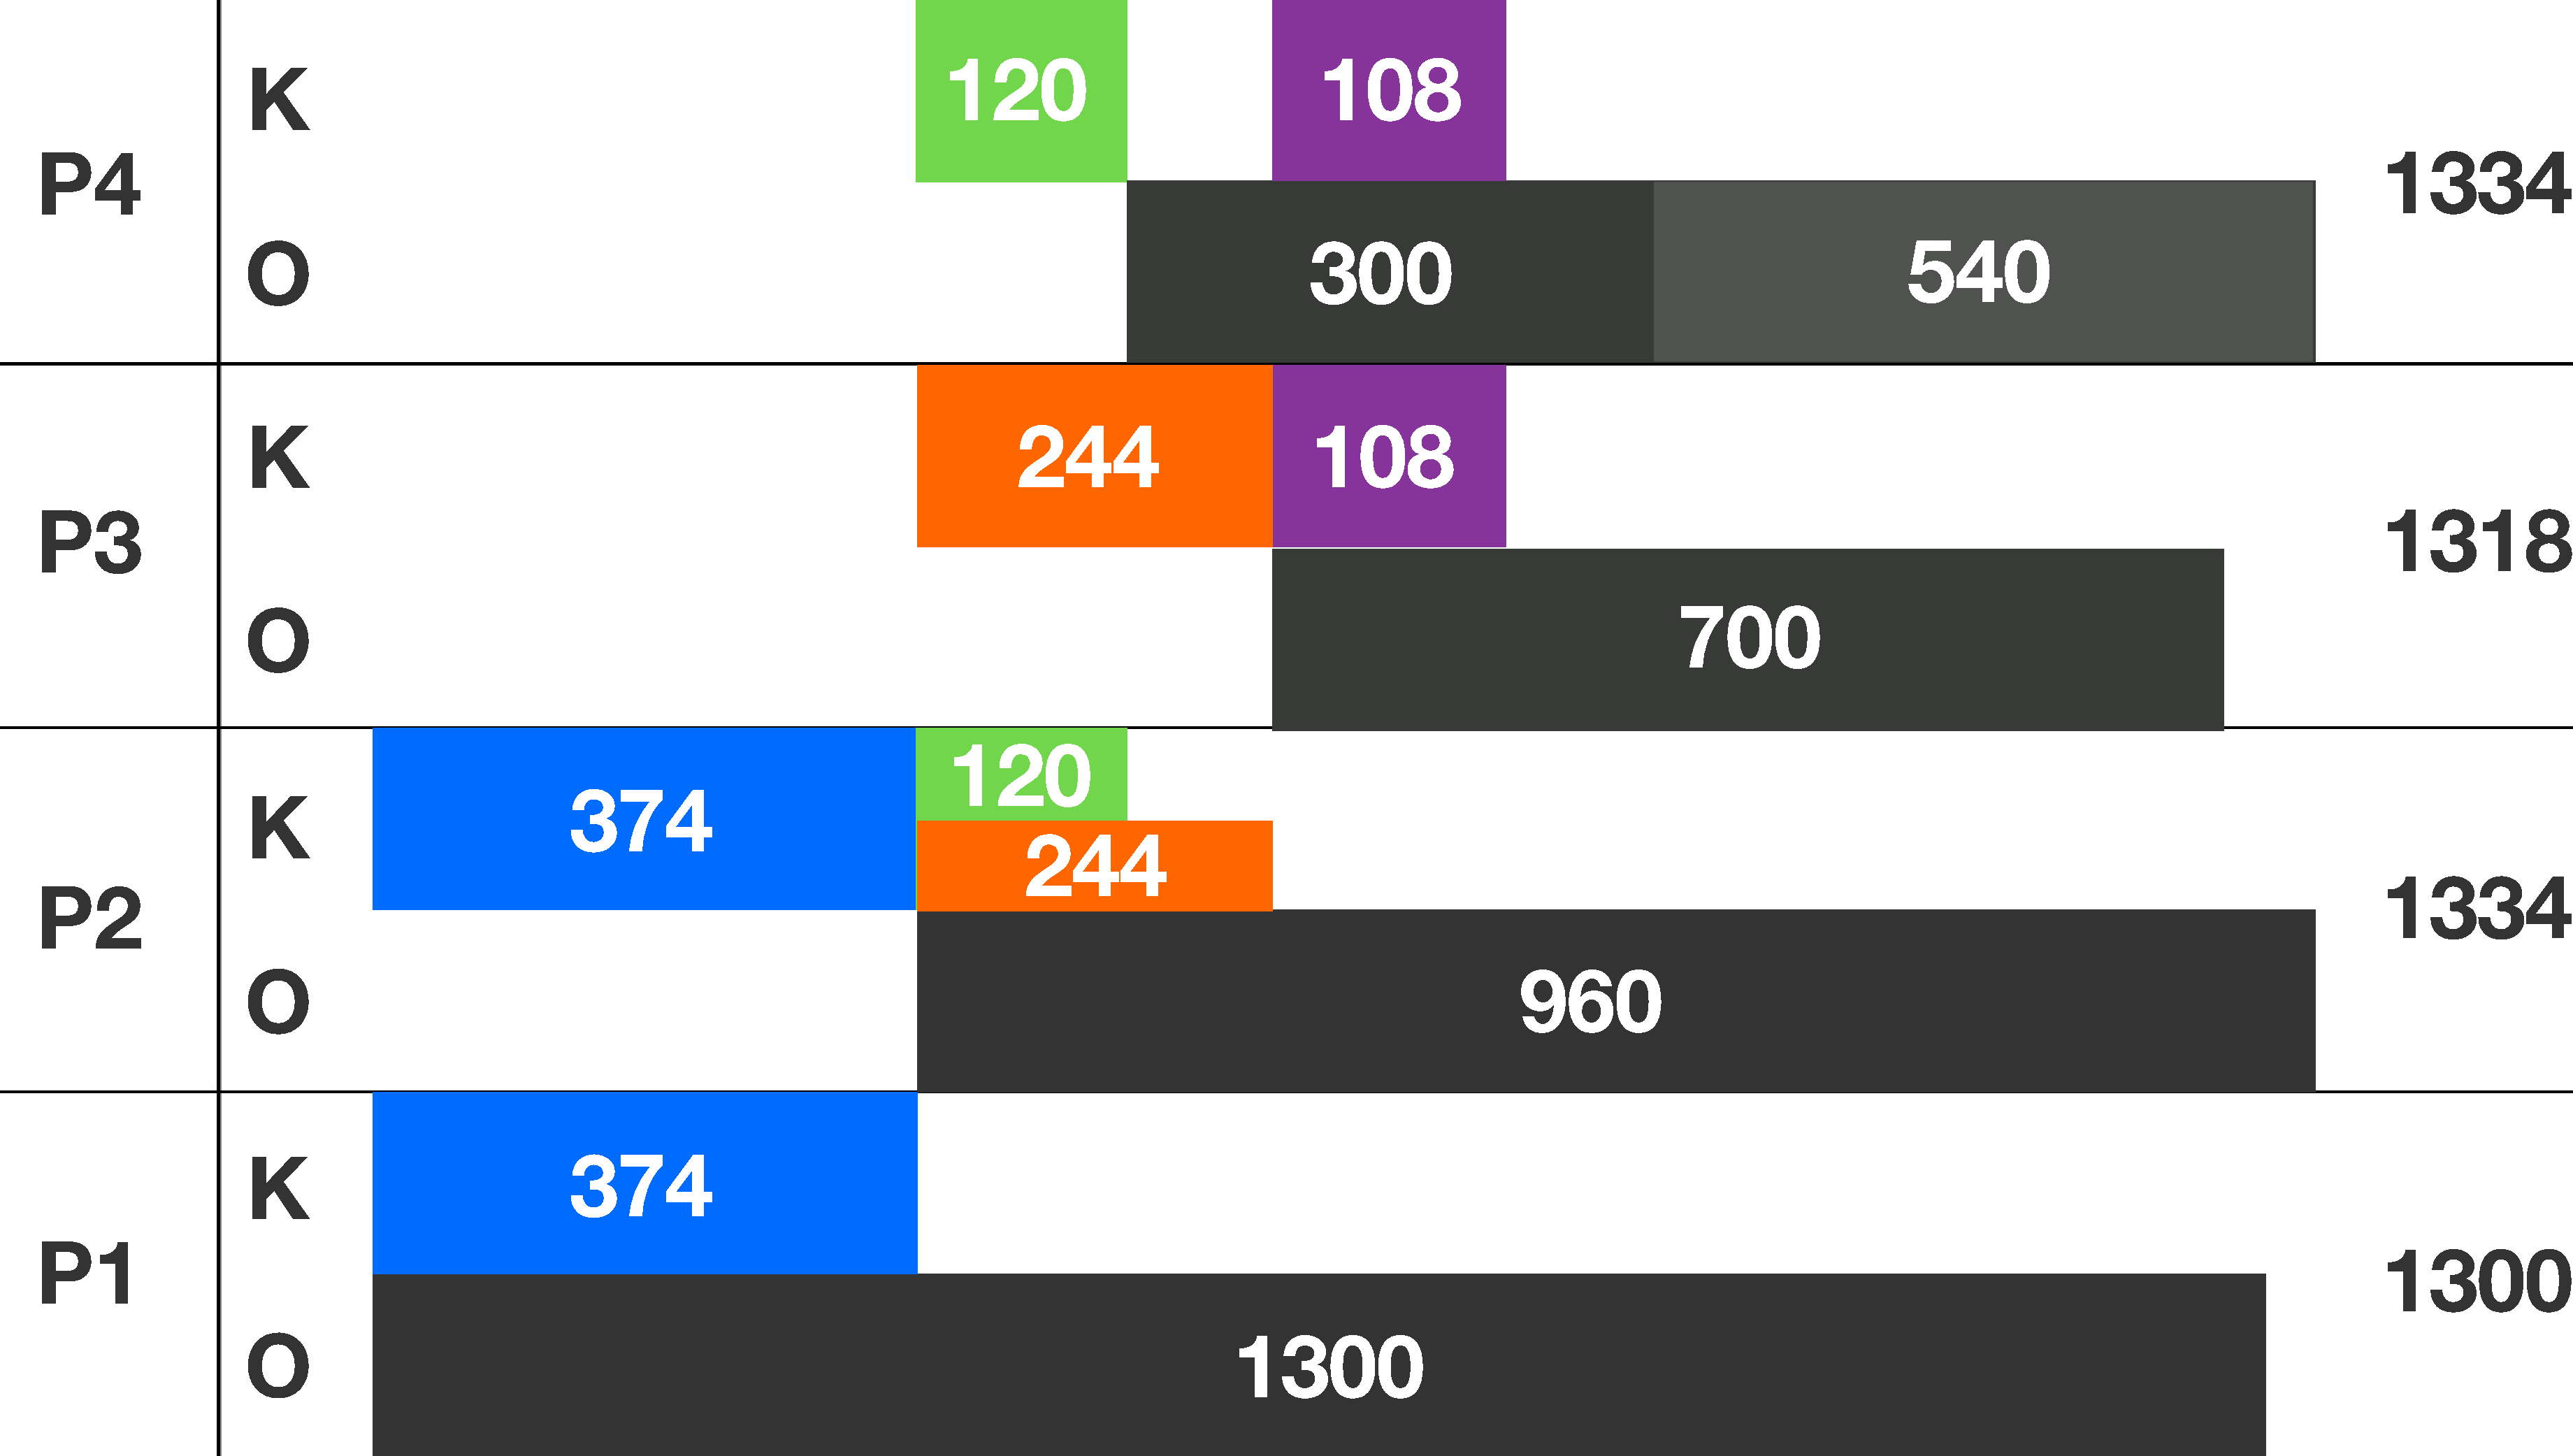
\includegraphics[width=1.0\textwidth]{g_par1.pdf}
\caption{Wykres Gantta dla testu~\ref{test4}}
\label{fig:res_4b}
\end{figure}

\subsection{Drugi test systemu równoległego} \label{test5}

\begin{table}[H]
\begin{minipage}[b]{0.5\linewidth}
\centering
\begin{tabular}{c l}
$V$ & 300 \\
$A1$ & 50 \\
$A2$ & 20 \\
$A3$ & 50 \\
$A4$ & 20 \\
$S12$ & 0 \\
$S23$ & 0 \\
$S34$ & 0 \\
$S24$ & 0 \\
$C12$ & 3 \\
$C23$ & 3 \\
$C34$ & 5 \\
$C24$ & 15 \\
\end{tabular}
\end{minipage}
\hspace{0.5cm}
\begin{minipage}[b]{0.5\linewidth}
\centering
\begin{tabular}{c l}
$T$ & 2933 \\
$d_{1}$ & 58 \\
$d_{2}$ & 110 \\
$d_{3}$ & 40 \\
$d_{4}$ & 92 \\
$d_{43}$ & 29 \\
$d_{42}$ & 63 \\
$t_{k12}$ & 726 \\
$t_{k23}$ & 207 \\
$t_{k24}$ & 945 \\
$t_{k34}$ & 145 \\
$bg24$ & 1 \\
\end{tabular}
\end{minipage}
\caption{Dane wejściowe i wyniki optymalizacji testu~\ref{test5}}
\label{tab:res_5a}
\end{table}

\begin{figure}[H]
\centering
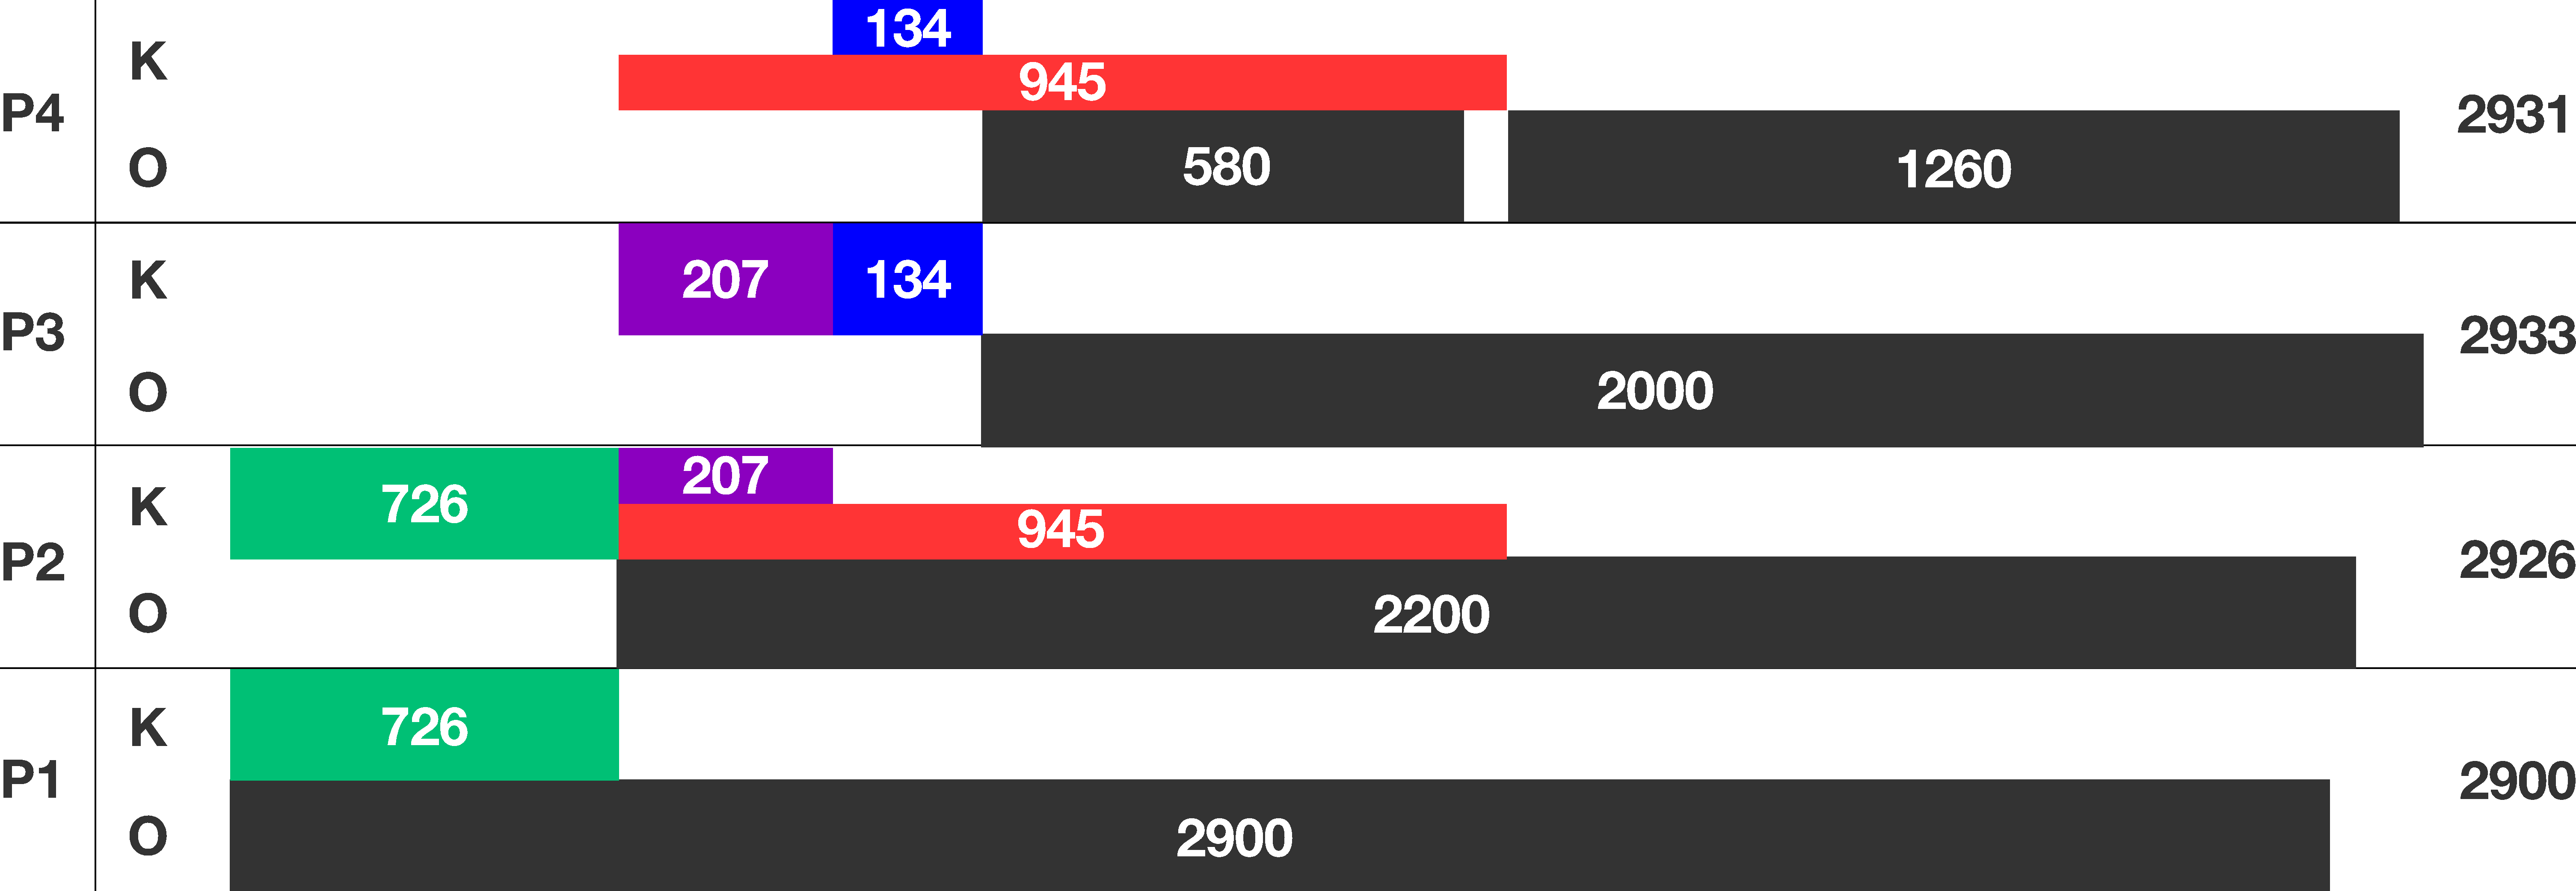
\includegraphics[width=1.0\textwidth]{g_par2.pdf}
\caption{Wykres Gantta dla testu~\ref{test5}}
\label{fig:res_5b}
\end{figure}

\newpage
